%  !TeX  root  =  user_guide.tex
% % \section{Print Composer}\label{label_printcomposer}
\chapter{Composeur de carte}\label{label_printcomposer}

% when the revision of a section has been finalized, 
% comment out the following line:
% \updatedisclaimer

%The print composer provides growing layout and printing
%capabilities. It allows you to add elements such as the QGIS map canvas, 
%legend, scalebar, images, and text labels. You can size, group 
%align and position each element and adjust the properties to create your
%layout. The layout can be printed or exported to image formats, Postscript,
%PDF or to SVG \footnote{Export to SVG supported, but it is not working
%properly with some recent QT4 versions. You should try and
%check individual on your system} and you can save the layout as template and
%load it again in another session. See a list of tools in
%table~\ref{tab:printcomposer_tools}:
Le composeur de carte fournit des fonctionnalités croissantes de mise en page et d'impression. Il vous permet d'ajouter des éléments tels qu'un cadre de carte QGIS, une légende, une échelle graphique, des images et des étiquettes. Vous pouvez modifier la taille, grouper , aligner et positionner chaque élément et ajuster leurs propriétés pour créer votre mise en page. Le résultat peut être imprimé ou exporté dans plusieurs formats d'images, mais aussi en Postscript, PDF et SVG.\footnote{L'export en SVG est géré, mais il ne fonctionne pas correctement avec certaines versions de QT4. Vous devriez essayer et vérifier indivuellement sur votre système} Voici une liste des outils (tableau~\ref{tab:printcomposer_tools}) :

\begin{table}[p]\index{Composeur de carte!outils}
\centering\small
\renewcommand{\arraystretch}{2}
 \begin{tabular}{|m{1cm}|m{5.4cm}|m{1cm}|m{5.4cm}|}
 \hline \textbf{Icône} & \textbf{Objectif} & \textbf{Icône} &
 \textbf{Objectif} \\
\hline 
\includegraphics[width=0.7cm]{mActionFolder} & Charger depuis un modèle &
 
\includegraphics[width=0.7cm]{mActionFileSaveAs} & Enregistrer en tant que modèle \\
\hline 
\includegraphics[width=0.7cm]{mActionExportMapServer}  & Exporter dans un format d'image & 
 
\includegraphics[width=0.7cm]{mActionSaveAsPDF} & Exporter en PDF \\
\hline 
\includegraphics[width=0.7cm]{mActionSaveAsSVG} & Exporter la composition en SVG& \multicolumn{2}{c|}{}\\
\hline 
\includegraphics[width=0.7cm]{mActionFilePrint} & Imprimer ou exporter en Postscript &
 
\includegraphics[width=0.7cm]{mActionZoomFullExtent} & Zoom à l'étendue maximale\\
\hline 
\includegraphics[width=0.7cm]{mActionZoomIn} & Zoom + &
 
\includegraphics[width=0.7cm]{mActionZoomOut} & Zoom - \\
\hline 
\includegraphics[width=0.7cm]{mActionDraw} & Rafraichie la vue &
 
\includegraphics[width=0.7cm]{mActionAddMap} & Ajouter une nouvelle carte à partir du cadre de carte de QGIS \\
\hline 
\includegraphics[width=0.7cm]{mActionSaveMapAsImage} & Ajouter une image au composeur de carte &
 
\includegraphics[width=0.7cm]{mActionLabel} & Ajoute des étiquettes à la composition de carte \\
\hline 
\includegraphics[width=0.7cm]{mActionAddLegend} & Ajoute une nouvelle légende à la composition de carte &
 
\includegraphics[width=0.7cm]{mActionScaleBar} & Ajoute une barre d'échelle graphique à la composition de carte\\
\hline 
\includegraphics[width=0.7cm]{mActionSelectPan} & Sélectionne/déplace les objets dans la composition de carte &
 
\includegraphics[width=0.7cm]{mActionMoveItemContent} & Déplace le contenu dans un objet \\
\hline 
\includegraphics[width=0.7cm]{mActionGroupItems} & Groupe les objets de la composition de carte & 
 
\includegraphics[width=0.7cm]{mActionUngroupItems} & Désolidaise les objets de la composition de carte \\
\hline 
\includegraphics[width=0.7cm]{mActionRaiseItems} & Passe les objets par dessus dans la composition de carte &
 
\includegraphics[width=0.7cm]{mActionLowerItems} & Passe les objets par dessous dans la composition de carte \\
\hline 
\includegraphics[width=0.7cm]{mActionMoveItemsToTop} & Déplace les objets sélectionnés tout en haut & 
 
\includegraphics[width=0.7cm]{mActionMoveItemsToBottom} & Déplace les objets sélectionnés tout en bas \\
 \hline 
\includegraphics[width=0.7cm]{mActionAlignLeft} & Aligner les objets sélectionnés à gauche &
 
\includegraphics[width=0.7cm]{mActionAlignRight} & Aligner les objets sélectionnés à droite \\
 \hline 
\includegraphics[width=0.7cm]{mActionAlignHCenter} & Aligner les objets sélectionnés au centre &
 
\includegraphics[width=0.7cm]{mActionAlignVCenter} & Aligner les objets sélectionnés au centre vertical \\
 \hline 
\includegraphics[width=0.7cm]{mActionAlignTop} & Aligner les objets sélectionnés vers le haut &
 
\includegraphics[width=0.7cm]{mActionAlignBottom} & Aligner les objets sélectionnés  vers le bas \\
\hline
\end{tabular}
\caption{Outils du Composeur de carte}\label{tab:printcomposer_tools}
\end{table}

% To access the print composer, click on the
% \toolbtntwo{mActionFilePrint}{Print} button in the toolbar or choose
% \mainmenuopt{File} > \dropmenuopttwo{mActionFilePrint}{Print Composer}.
Pour accéder au composeur de carte, cliquez sur le bouton \toolbtntwo{mActionFilePrint}{Imprimer} dans la barre d'outils ou choisissez \mainmenuopt{Fichier} > \dropmenuopttwo{mActionFilePrint}{Composeur de carte}.

% \section{Using Print Composer}\label{label_useprintcomposer} 
\section{Utiliser le Composeur d'Impression}\label{label_useprintcomposer} 


% Before you start to work with the print composer, you need to load some 
% raster and vector layers in the QGIS map canvas and adapt their properties 
% to suite your own convinience. After everything is rendered and symbolized to 
% your liking you click the \toolbtntwo{mActionFilePrint}{Print Composer} icon.
Avant de démarrer à travailler avec le composeur de carte, vous devez charger certaines couches raster et vecteurs dans la fenêtre de carte de QGIS et 
adapter leurs propriétés pour qu'elles vous conviennent. Après que tout soit rendu et symbolisé comme vous le souhaitez, cliquez sur l'icône \toolbtntwo{mActionFilePrint}{Composeur de carte}.

%\begin{figure}[ht]
%   \begin{center}
%   \caption{Print Composer \nixcaption}\label{fig:print_composer_blank}\smallskip
%   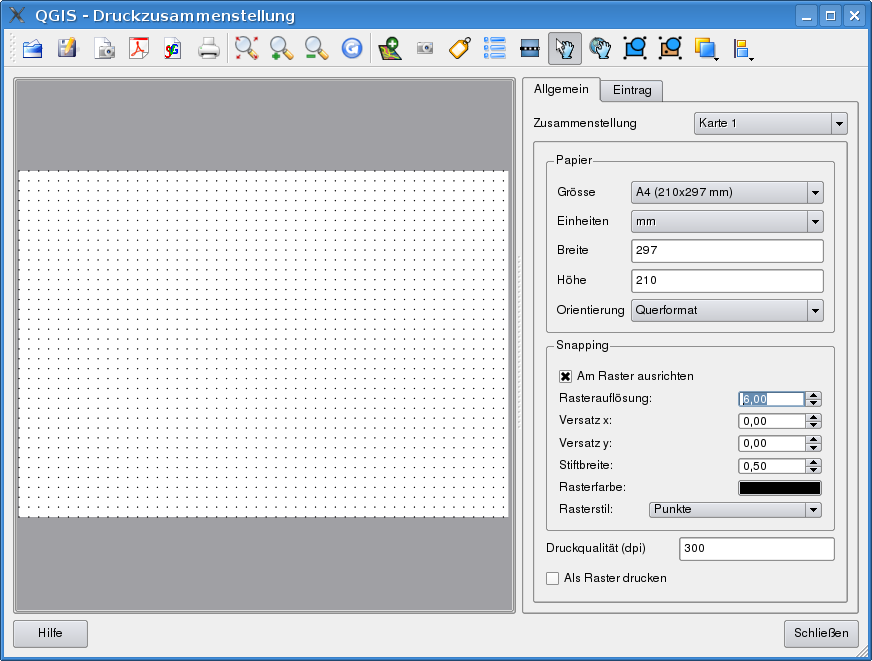
\includegraphics[clip=true, width=\textwidth]{print_composer_blank}
%\end{center}  
%\end{figure}

\begin{figure}[ht]
   \begin{center}
   \caption{Composeur de carte\nixcaption}\label{fig:print_composer_blank}\smallskip
   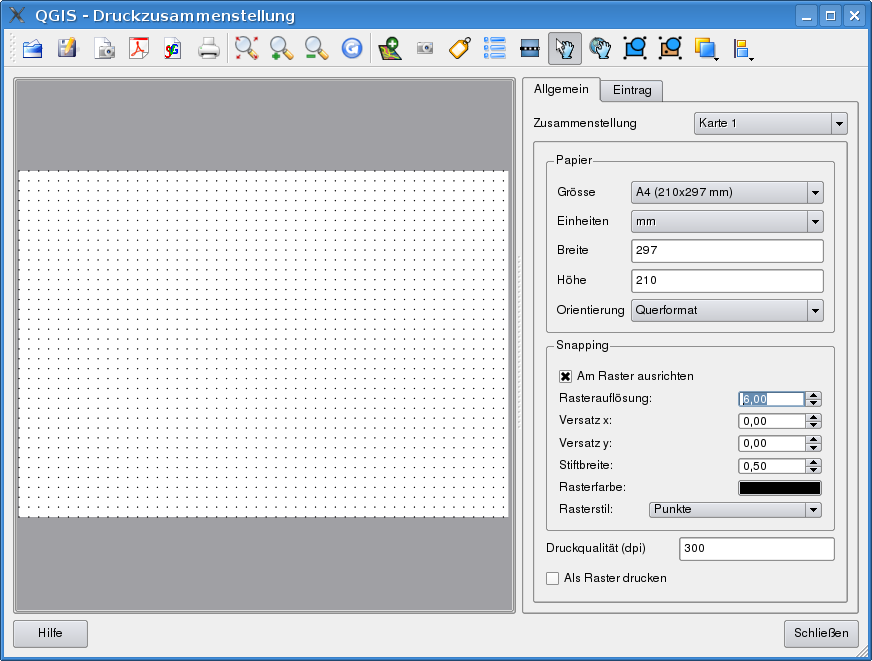
\includegraphics[clip=true, width=10cm]{print_composer_blank}
\end{center}
\end{figure}

% Opening the print composer provides you with a blank canvas to which you can 
% add the current QGIS map canvas, legend, scalebar, images and text. Figure
% \ref{fig:print_composer_blank} shows the initial view of the print composer 
% before any elements are added. The print composer provides two tabs:
Ouvrir le composeur de carte vous affiche un cadre vide auquel vous pouvez ajouter un cadre de la carte actuelle de QGIS, une légende, une échelle
graphique, des images et du texte. La figure \ref{fig:print_composer_blank} montre la vue initiale du composeur de carte avant qu'un élément ne soit ajouté. Le composeur de carte affiche deux onglets :

\begin{itemize}[label=--]
%\item The \tab{General} tab allows you to set paper size, orientation, the
%print quality for the output file in dpi and to activate snapping to a grid
%of a defined resolution. Please note, the \checkbox{Snap to grid} feature
%only works, if you define a grid resolution > 0. Furthermore you can also
%activate the \checkbox{Print as raster} checkbox. This means all elements
%will be rastered before printing or saving as Postscript of PDF.
\item l'onglet \tab{Général} vous permet de définir la taille du papier, l'orientation et la qualité d'impression pour le fichier de sortie (en dpi/ppp) et d'activer l'accrochage sur une grille d'une résolution prédéfinie. La fonction \checkbox{Accrochage à la grille} marche uniquement si vous avez défini une résolution supérieure à 0. Vous pouvez activer la case\\ \checkbox{Imprimer en tant que raster} qui permet de rastériser tous les éléments avant l'impression ou l'export.
%\item The \tab{Item} tab displays the properties for the selected map
%element. Click the \toolbtntwo{mActionSelectPan}{Select/Move item} 
%icon to select an element (e.g. legend, scalebar or label) on the canvas. 
%Then click the Item tab and customize the settings for the selected element.
\item L'onglet \tab{Item} affiche les propriétés pour l'élément de la carte sélectionnée. Cliquez sur l'icône \toolbtntwo{mActionSelectPan}{Sélectionner/Déplacer l'objet}  pour sélectionner un élément (par exemple l'échelle graphique ou une étiquette) dans le cadre. Puis cliquez sur l'onglet Item et personnalisez les paramètres pour l'élément sélectionné.
\end{itemize}

% You can add multiple elements to the composer. It is also possible to have 
% more than one map view or legend or scalebar in the print composer canvas. 
% Each element has its own properties and in the case of the map, its own 
% extent.
Vous pouvez ajouter de multiples éléments au composeur. Il est également possible d'avoir plus d'une vue de carte, légende ou échelle graphique dans le
cadre du composeur de carte. Chaque élément possède ses propres propriétés et dans le cas de la carte, sa propre étendue.

% \subsection{Adding a current QGIS map canvas to the Print Composer}
\subsection{Ajouter une carte en cours dans QGIS au Composeur d'Impression}

%To add the QGIS map canvas, click on the \toolbtntwo{mActionAddMap}{Add new map 
%from QGIS map canvas} button in the print composer toolbar and drag a 
%rectangle on the composer canvas with the left mouse button to add the map. 
%You will see an empty box with a \textit{"Map will be printed here"} message.
Pour ajouter le cadre de carte de QGIS, cliquez sur le bouton\\ \toolbtntwo{mActionAddMap}{Ajouter une nouvelle carte à partir du
cadre de carte de QGIS} dans la barre d'outils du composeur de carte et dessinez un rectangle dans le cadre du composeur avec le bouton gauche de la souris pour ajouter la carte. Vous verrez une boîte vide avec un message \og\textit{ La carte sera imprimée ici}\fg. Pour afficher la carte actuelle, choisissez
\selectstring{Preview}{Cache} dans l'onglet \tab{Item} de la carte.
%To display the current map, you can choose between three different modes in
%the map \tab{Item} tab:
Pour ajouter la carte courante, vous devez choisir entre 3 différentes modes dans l'onglet \tab{Item} :

%\begin{itemize}
%\item \selectstring{Preview}{Rectangle} is the default setting. It only
%displays an empty box with a message \textit{"Map will be printed here"}. 
%\item \selectstring{Preview}{Cache} renders the map in the current screen
%resolution. If case you zoom in or out the composer window, the map is not
%rendered again but the image will be scaled.
%\item \selectstring{Preview}{Render} means, that if you zoom in or out the
%composer window, the map will be rendered again, but for space reasons, only
%up to a maximum resolution.
%\end{itemize}

\begin{itemize}[label=--]
\item \selectstring{Aperçu}{Rectangle} est le paramètre par défaut. Il n'affiche qu'une boîte vide avec le message \og\textit{La carte sera imprimée ici}\fg. 
\item \selectstring{Aperçu}{Cache} affiche la carte dans sa résolution d'écran actuelle. Si vous zoomez sur la fenêtre de composition, la carte ne sera pas actualisée, mais l'image sera mise à l'échelle.
\item \selectstring{Aperçu}{Rendu} signifie que si vous faites un zoom dans la fenêtre de composition la carte sera actualisée, mais pour des raisons de performances, seulement jusqu'à une résolution maximum prédéfinie par QGIS.
\end{itemize}

\begin{figure}[ht]
\centering
% \caption{Print Composer map item tab content
% \nixcaption}\label{fig:print_composer_map_item}

   \subfloat[Width, height and extend dialog]
{\label{subfig:print_composer_map_item1}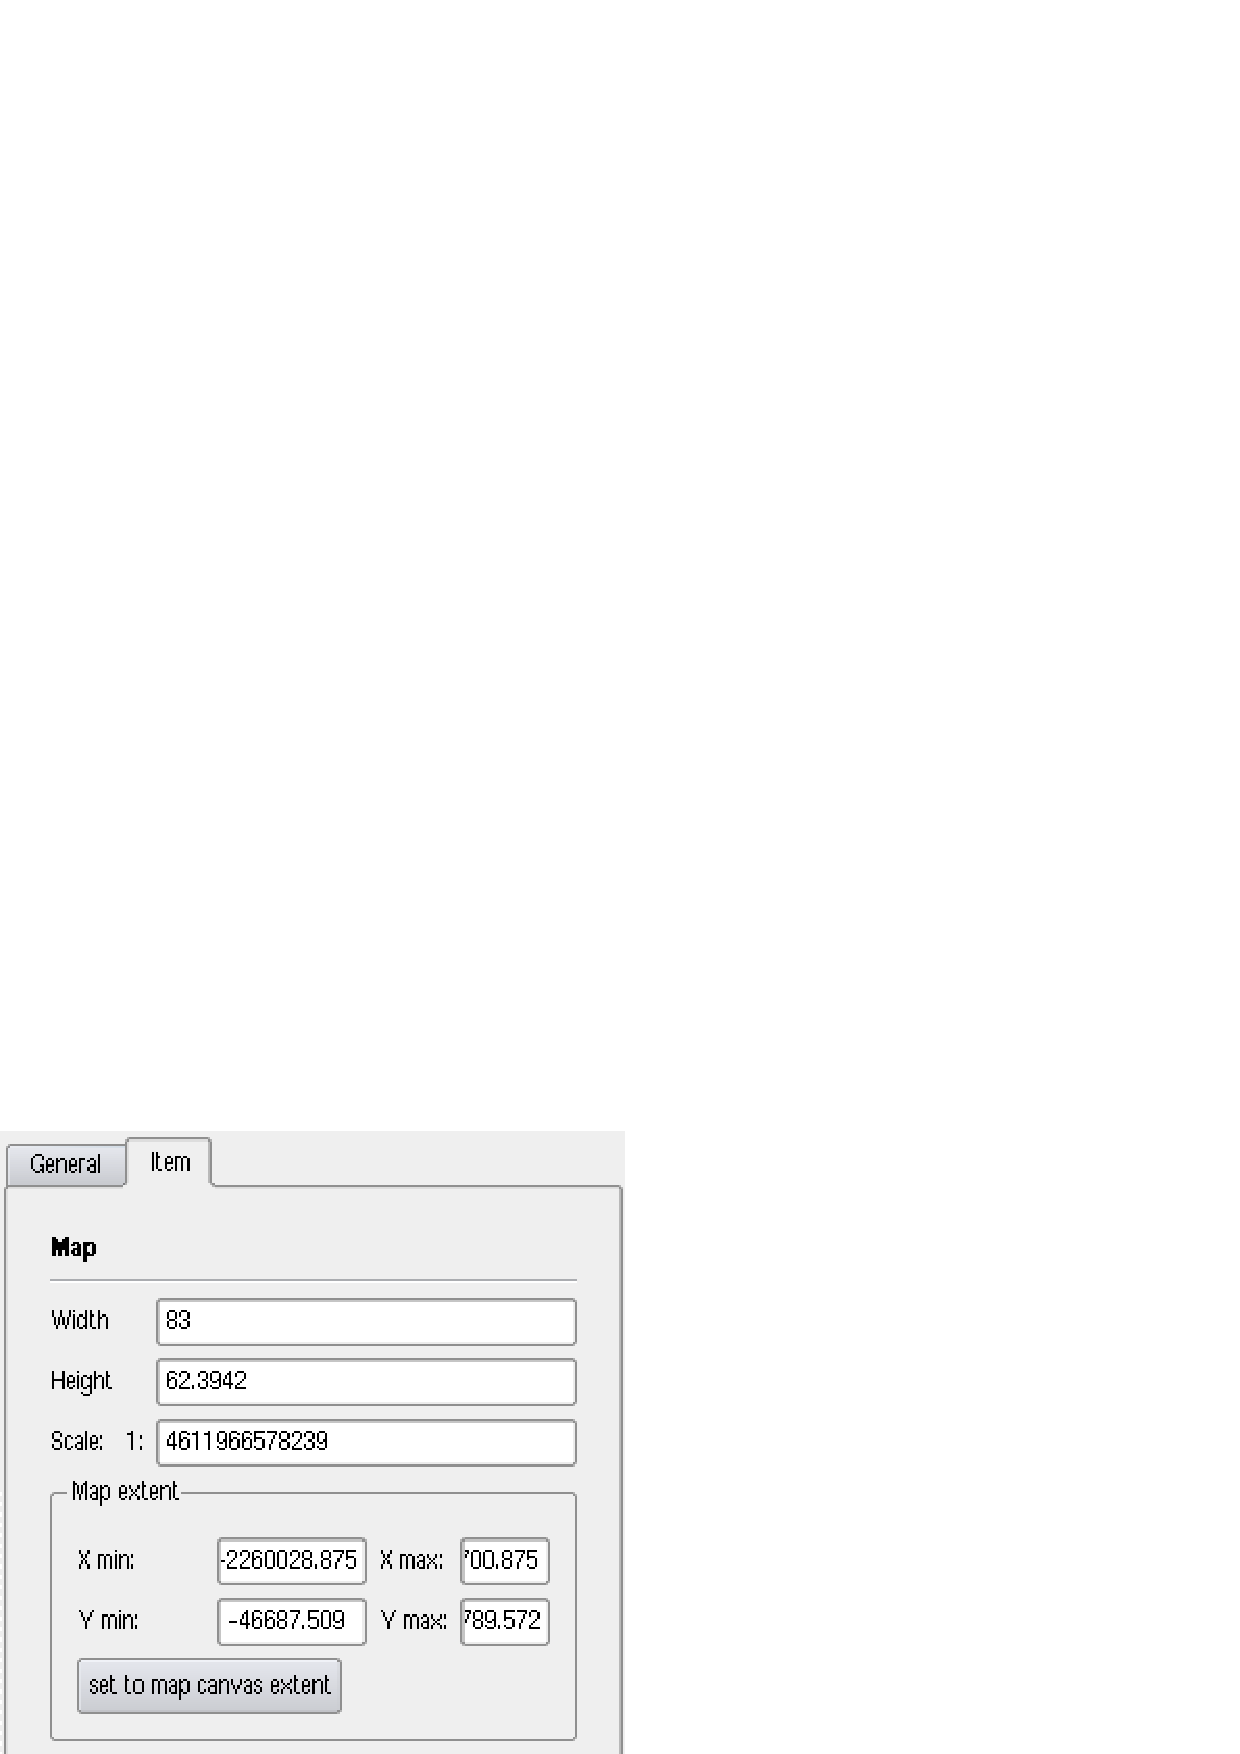
\includegraphics[clip=true,
width=0.4\textwidth]{print_composer_map_item1}}
% \subfloat[Properties dialog]
\hspace{0.5cm}
   \subfloat[Boîte de dialogue des propriétés]{\label{subfig:print_composer_map_item2}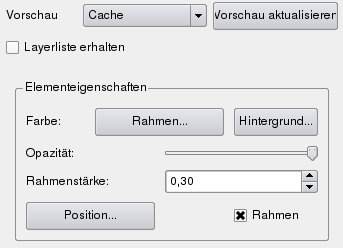
\includegraphics[clip=true,width=0.4\textwidth]{print_composer_map_item2}}
   \caption{L'onglet Item de la carte dans le composeur de carte
\nixcaption}\label{fig:print_composer_map_item}
\end{figure}

%You can resize the map later by clicking on the
%\toolbtntwo{mActionSelectPan}{Select/Move item} button, selecting the
%element, and dragging one of the blue handles in the corner of the map. With
%the map selected, you can now adapt more properties in the map \tab{Item}
%tab. Resize the map item specifying the width and height or the scale. Define
%the map extend using Y and X min/max values or clicking the \button{set to
%map canvas extend} button. Update the map preview and select, whether to see
%a preview from cache or an empty rectangle with a \textit{"Map will be
%printed here"} message. Define colors and outline width for the element
%frame, set a background color and opacity for the map canvas. And you can
%also select or unselect to display an element frame with the \checkbox{frame}
%checkbox (see Figure~\ref{fig:print_composer_map_item}). If you change the
%view on the QGIS map canvas by zooming or panning or changing vector or
%raster properties, you can update the print composer view selecting the map
%element in the print composer and clicking the \button{Update Preview} button
%in the map \tab{Item} tab (see Figure~\ref{fig:print_composer_map_item}). 

Vous pouvez redimensionner la carte plus tard en cliquant sur le bouton\\ \toolbtntwo{mActionSelectPan}{Sélectionner/Déplacer l'objet}, en sélectionnant
l'élément, et en déplaçant un des curseurs bleus dans le coin de la carte. Avec la carte sélectionnée, vous pouvez maintenant adapter plus de propriétés dans l'onglet \tab{Item} de la carte. Redimensionnez la carte en spécifiant la largeur et la hauteur ou l'échelle. Définissez l'étendue de la carte en utilisant les valeurs min/max pour X et Y, ou en cliquant le bouton \button{Fixer sur l'emprise courante}. Faites une mise à jour de l'aperçu de la carte et sélectionnez, soit pour voir un aperçu du cache ou un rectangle vide. Définissez les couleurs et les épaisseurs de bordure pour les cadres des éléments, mettez une couleur d'arrière-plan. Vous pouvez aussi choisir d'afficher ou pas un cadre d'élément avec la case \checkbox{cadre} (see Figure~\ref{fig:print_composer_map_item}). Si vous changez la vue sur la carte principale de QGIS en zoomant, en vous déplaçant ou en changeant des propriétés d'affichage, vous pouvez mettre à jour la vue du composeur en cliquant sur le bouton \button{Mise à jour de l'aperçu} dans l'onglet \tab{Item} (voir figure~\ref{fig:print_composer_map_item}). 

% To move layers within the map element select the map element, click 
% the \toolbtntwo{mActionMoveItemContent}{Move item content} icon and move the
% layers within the map element frame with the left mouse button.
Pour déplacer une couche dans l'élément de la carte, sélectionnez-le puis cliquez sur l'icône \toolbtntwo{mActionMoveItemContent}{Déplacer le contenu de l'objet} et déplacez les couches dans le cadre de l'élément 'carte' avec le bouton gauche de la souris.
%After you found the right place for an element, you can lock the element
%position within the print composer canvas. Select the map element and click
%on the right mouse button to \toolbtntwo{mIconLock}{lock} the element
%position and again to unlock the element.
Après avoir trouvé le bon emplacement, vous pouvez figer la position de cet élément au sien du composeur. Sélectionnez l'élément, faites un clic droit et choisissez \toolbtntwo{mIconLock}{verrouiller}.

%\subsection{Navigation tools}
\subsection{Outils de navigation}

%For map navigation the print composer provides 4 general tools:
Pour naviguer sur la carte, le composeur propose 4 outils généralistes /

%\begin{itemize}
%\item \toolbtntwo{mActionZoomOut}{Zoom in},
%\item \toolbtntwo{mActionZoomOut}{Zoom out},
%\item \toolbtntwo{mActionZoomFullExtent}{Zoom to full extend} and
%\item \toolbtntwo{mActionDraw}{Refresh the view}, if you find the view in an
%inconsistent state.
%\end{itemize}
\begin{itemize}[label=--]
\item \toolbtntwo{mActionZoomOut}{Zoom +}
\item \toolbtntwo{mActionZoomOut}{Zoom -}
\item \toolbtntwo{mActionZoomFullExtent}{Zoomer sur l'emprise maximale}
\item \toolbtntwo{mActionDraw}{RActualiser l'aperçu}
\end{itemize}

% \subsection{Adding other elements to the Print Composer}
\subsection{Ajouter d'autres éléments au Composeur d'Impression}

%Besides adding a current QGIS map canvas to the Print Composer, it is also possible 
%to add, position, move and customize legend, scalebar, images and label elements.
Au-delà de l'ajout d'un cadre de la carte actuelle de QGIS au composeur de carte, il est également possible d'ajouter, déplacer et personnaliser les
éléments légendes, échelles graphiques, images et étiquettes.

% \minisec{Label and images}
\minisec{Étiquette et images}

%To add a label or an image, click the \toolbtntwo{mActionLabel}{Add label} or 
%\toolbtntwo{mActionSaveMapAsImage}{Add image} icon, place the element with
%the left mouse button on the print composer canvas and position and customize
%their appearance in the \tab{Item} tab.
Pour ajouter une étiquette ou une image, cliquez sur l'icône\\ \toolbtntwo{mActionLabel}{Ajouter une étiquette} ou \toolbtntwo{mActionSaveMapAsImage}{Ajouter une image} et placez l'élément avec le bouton gauche de la souris sur le cadre du composeur de carte, modifiez leur apparence avec l'onglet \tab{Item}.

\begin{figure}[p]
\centering
% \caption{Customize print composer label and images

%    \subfloat[label item tab]
   \subfloat[onglet item des étiquettes]
{\label{subfig:print_composer_label_item}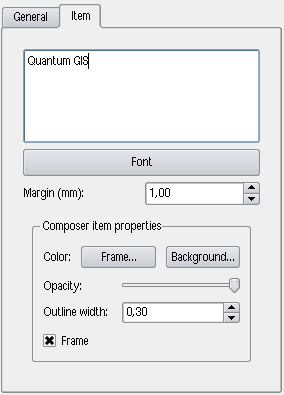
\includegraphics[clip=true,
width=0.4\textwidth]{print_composer_label_item}}
%    \subfloat[image item tab]
\hspace{0.5cm}
   \subfloat[onglet item des images]
{\label{subfig:print_composer_image_item}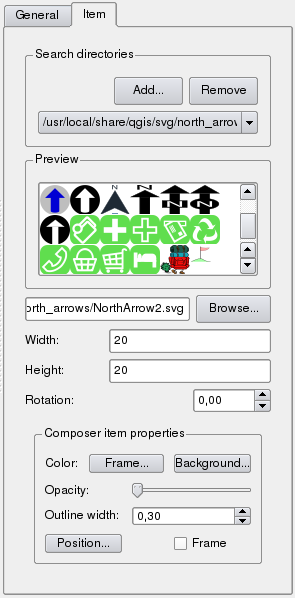
\includegraphics[clip=true,
width=0.4\textwidth]{print_composer_image_item}}
\caption{Personnaliser les étiquettes et les images du composeur de carte
\nixcaption}\label{fig:print_composer_tab2}
\end{figure}

% \minisec{Legend and scalebar}
\minisec{Légende  et barre d'échelle}

% To add a map legend or a scalebar, click the \toolbtntwo{mActionAddLegend}{Add
% new legend} or \toolbtntwo{mActionScaleBar}{Add new scalebar} icon and place
% the element with the left mouse button on the print composer canvas.

%To add a map legend or a scalebar, click the \toolbtntwo{mActionAddLegend}{Add new legend} or 
%\toolbtntwo{mActionScaleBar}{Add new scalebar} icon, place the element with the left 
%mouse button on the print composer canvas and position and customize their appearance in the \tab{Item} tab.

Pour ajouter une légende ou une échelle graphique, cliquez sur l'icône\\ \toolbtntwo{mActionAddLegend}{ajouter une nouvelle légende} ou \toolbtntwo{mActionScaleBar}{Ajouter une nouvelle échelle graphique}, placez l'élément avec le bouton gauche de la souris sur le cadre du composeur de carte et modifiez leur apparence avec l'onglet \tab{Item}.

\begin{figure}[ht]
\centering
% \caption{Customize print composer legend and scalebar

%    \subfloat[legend item tab]
    \subfloat[onglet item de la légende]
{\label{subfig:print_composer_legend_item}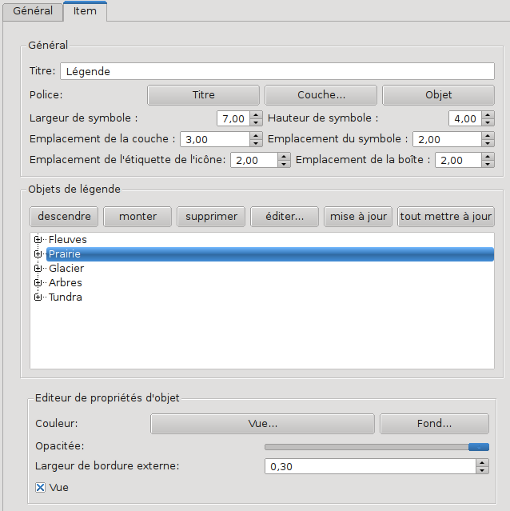
\includegraphics[clip=true,
width=0.4\textwidth]{print_composer_legend_item}}
%    \subfloat[scalebar item tab]
\hspace{0.5cm}
      \subfloat[onglet item de l'échelle graphique]
{\label{subfig:print_composer_scalebar_item}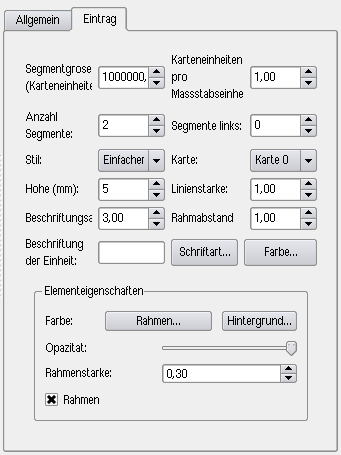
\includegraphics[clip=true,
width=0.4\textwidth]{print_composer_scalebar_item}}
\caption{Personnaliser la légende et l'échelle graphique du composeur de carte
\nixcaption}\label{fig:print_composer_tab1}
\end{figure}

%\subsection{Raise, lower and align elements}
\subsection{Monter, descendre et aligner des éléments}

%Raise or lower functionalities for elements are inside the
%\toolbtntwo{mActionRaiseItems}{Raise selected items} pulldown menu. Choose an
%element on the print composer canvas and select the matching functionality to
%raise or lower the selected element compared to the other elements (see
%table~\ref{tab:printcomposer_tools}). 
Les fonctionnalités pour relever ou descendre des éléments sont présentes dans le menu déourlant \toolbtntwo{mActionRaiseItems}{Relever les objets sélectionnés}. Prenez un élément dans le composeur de carte et sélectionnez la fonction correspondante pour le relever ou le descendre par rapport aux autres éléments (voir table~\ref{tab:printcomposer_tools}).

%There are several alignment functionalities available within the
%\toolbtntwo{mActionAlignLeft}{Align selected items} pulldown menu (see
%table~\ref{tab:printcomposer_tools}). To use an alignment functionality , you
%first select some elements and then click on the matching alignment icon. All
%selected will then be aligned within to their common bounding box.
Il y a plusieurs fonctionnalités d'alignements disponibles dans le menu déroulant\\ \toolbtntwo{mActionAlignLeft}{Aligner les objets sélectionnés} (voir table~\ref{tab:printcomposer_tools}). Pour utiliser une fonction, vous devez d'abord sélectionner plusieurs éléments et ensuite cliquer sur l'icône d'alignement désiré. Toute la sélection sera alignée dans le cadre de leurs limites respectives

% \subsection{Creating Output}
\subsection{Création de carte}

% Figure \ref{fig:print_composer_complete} shows the print composer with an
% example print layout including each type of map element described in the
% sections above.
La figure \ref{fig:print_composer_complete} montre le composeur de carte avec
un exemple de mise en page incluant chaque type d'élément de la carte décrit
dans la section au-dessus.

\begin{figure}[ht]
   \begin{center}
%    \caption{Print Composer with map view, legend, scalebar, and text added
\smallskip
   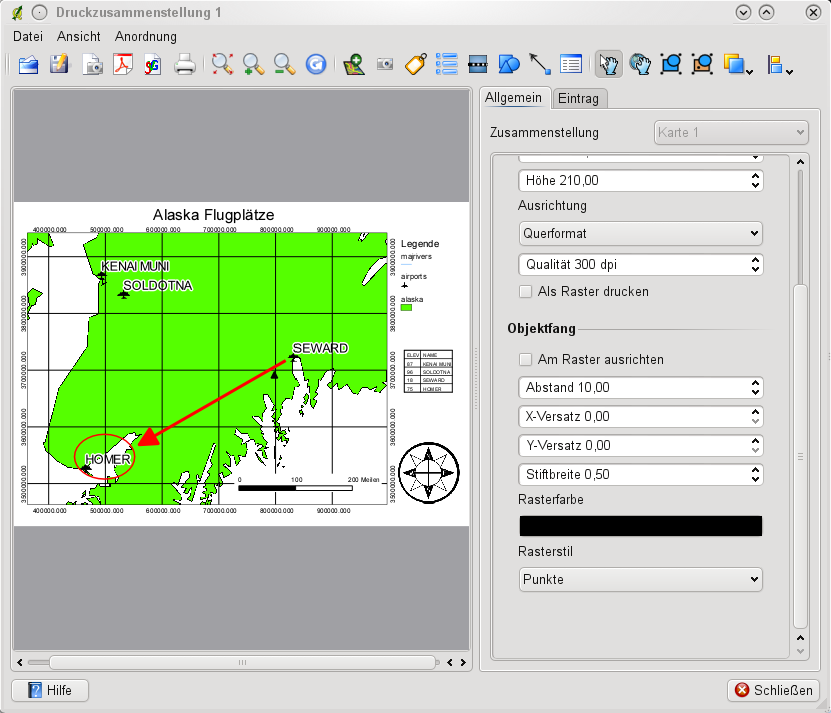
\includegraphics[clip=true, width=\textwidth]{print_composer_complete}
   \caption{Composeur de carte avec une vue de la carte, de la légende, de
l'échelle graphique et du texte ajouté \nixcaption}
   \label{fig:print_composer_complete}
\end{center}
\end{figure}

% The print composer allows you to create several output formats and it is
% possible to define the resolution (print quality) and paper size:
Le composeur de carte vous permet de choisir plusieurs formats de sortie et il est possible de définir la résolution (qualité d'impression) et la taille du papier :

\begin{itemize}[label=--]
% \item The \toolbtntwo{mActionFilePrint}{Print} icon allows to print the
% layout to a connected printer or as PDF or Postscript file depending on
% installed printer drivers.
\item L'icône \toolbtntwo{mActionFilePrint}{Imprimer}  permet d'imprimer la mise en page à une imprimante ou dans un fichier Postscript en fonction des pilotes d'imprimante installés.
%\item The \toolbtntwo{mActionSaveAsPDF}{Export as PDF} saves the defined
%print composer canvas directly as a PDF.
\item The \toolbtntwo{mActionSaveAsPDF}{Exporter au format PDF} enregistre le contenu du composeur directement dans un fichier PDF.
% \item The \toolbtntwo{mActionExportMapServer}{Export as image} icon exports
% the composer canvas in several image formats such as PNG, BPM, TIF, JPG, \dots
\item L'icône \toolbtntwo{mActionExportMapServer}{Exporter dans une image} exporte le cadre du composeur dans plusieurs formats d'image tels que PNG, BPM,TIF, JPG, \dots

% \item The \toolbtntwo{mActionSaveAsSVG}{Export as SVG} icon saves the print 
% composer canvas as a SVG (Scalable Vector Graphic). \textbf{Note:} Currently
% the SVG output is very basic. This is not a QGIS problem, but a problem of the
% underlaying Qt library. This will hopefully be sorted out in future versions.
\item L'icône \toolbtntwo{mActionSaveAsSVG}{Exporter au format SVG} sauve le cadre du composeur de carte en SVG (Scalable Vector Graphic). \textbf{Note :} Actuellement la sortie SVG est très basique. Ce n'est pas un problème de QGIS mais un problème de la bibliothèque Qt sous-jacente. Cela sera
probablement corrigé dans une prochaine version. \end{itemize}

%\subsection{Saving and loading a print composer layout}
\subsection{Enregistrer et charger une mise en page d'impression}

%With the \toolbtntwo{mActionFileSaveAs}{Save as template} and
%\toolbtntwo{mActionFolder}{Load from template} icons you can save the current
%state of a print composer session as a  *.qpt template and load the template
%again in another session.
Avec les icônes \toolbtntwo{mActionFileSaveAs}{Sauvegarder en tant que modèle} et \toolbtntwo{mActionFolder}{Charger depuis un modèle}, vous pouvez enregistrer l'état actuel d'une session du composeur dans un modèle *.qpt et le charger dans une autre session.
